\section{Circuit implementations}

\begin{frame}[c]{Hypergraph product codes}
  \centering
  \hfill \\[5mm]
  \begin{tikzpicture}
    \onslide<3> {
      \fill[spinsecondarylighter] (1.7, -1) rectangle (2.8, 6.5);
    }

    \onslide<4> {
      \fill[spinsecondarylighter] (-0.5, 2.2) rectangle (7, 3.3);
    }

    \onslide<3-> {

      \foreach \x in {0,..., 6}
        \draw (\x + 0.5, -0.5) -- (\x + 0.5, 5.5);
      \foreach \y in {0,..., 6}
        \draw (0.5, \y-0.5) -- (6.5, \y - 0.5);
      \foreach \x in {0,..., 6}
        \foreach \y in {0,..., 6}
          \draw (\x + 0.5, \y - 0.5) -- (\x, \y);

    }

    \onslide<2> {
      \fill[spinsecondarylighter] (1.5, -0.5) rectangle (2.5, 6.5);
      \fill[spinsecondarylighter] (-0.5, 2.5) rectangle (6.5, 3.5);
    }

    \foreach \x in {0,..., 3}
      \foreach \y in {0,..., 3}
        \draw[spinprimary, line width=0.15em, fill=white] (2*\x, 2*\y) circle (0.1);

    \foreach \x in {0,..., 2}
      \foreach \y in {0,..., 2}
        \draw[spinprimary, line width=0.15em, fill=white] (1 + 2*\x, 1 + 2*\y) circle (0.1);

    \foreach \x in {0, ..., 2}
      \foreach \y in {0, ..., 3}
        \draw[spinsecondary, line width=0.15em, fill=white] (1 + 2*\x - 0.1, 2*\y - 0.1) rectangle (1 + 2*\x + 0.1, 2*\y + 0.1);

    \foreach \x in {0, ..., 3}
      \foreach \y in {0, ..., 2}
        \draw[spinsecondary, line width=0.15em, fill=white] (2*\x - 0.1, 1 + 2*\y - 0.1) rectangle (2*\x + 0.1, 1 + 2*\y + 0.1);

    \onslide<2-> {
        \fill[spinsecondary] (2 - 0.1, 3 - 0.1) rectangle (2+ 0.1, 3 + 0.1);
    }

    \onslide<2-> {
        \fill[spinprimary] (2, 0) circle (0.1);
        \fill[spinprimary] (2, 2) circle (0.1);
        \fill[spinprimary] (2, 6) circle (0.1);
        \fill[spinprimary] (1, 3) circle (0.1);
        \fill[spinprimary] (5, 3) circle (0.1);
    }

    \onslide<3-> {
      \foreach \x in {0,..., 6}
        \foreach \y in {0,..., 6}
          \node
            [diamond, draw = spinternary, fill=white, scale=0.6, line width=0.15em] 
              (d_\x_\y) at (\x + 0.5, \y - 0.5) {};

      \foreach \x in {0,..., 6}
        \node
        [diamond, fill = spinternary, scale=0.6, line width=0.15em] 
          (a_\x) at (0.5 + \x, 2.5) {};

      \foreach \y in {0,..., 6}
        \node
        [diamond, fill = spinternary, scale=0.6, line width=0.15em] 
          (b_\y) at (2.5, \y - 0.5) {};
    }
  \end{tikzpicture}
\end{frame}

\begin{frame}[c]
    \centering 
    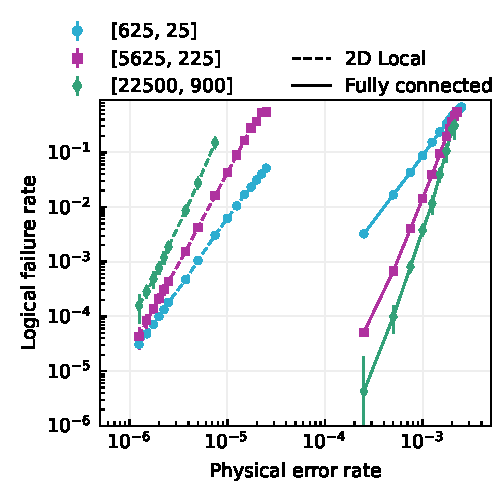
\includegraphics{figs/comparison_alt.pdf}
\end{frame}

\begin{frame}[c]{Comparison to surface code}
  \centering
  \begin{tabular} { l c c c }
      Logical failure rate & $10^{-9}$ & $10^{-12}$ & $10^{-15}$ \\
      \hline
      Logical qubits & \num{1600} & \num{6400} & \num{18496} \\
%            Surface code distance  & \num{11} & \num{15}  & \num{19} \\
      Surface code physical qubits & \num{387200} & \num{2880000}  & \num{13354112} \\
      HGP code physical qubits & \num{78400}   & \num{313600}   & \num{906304} \\
      Improvement using HGP codes & \num{4.94}$\times$   & \num{9.18}$\times$  & \num{14.73}$\times$ \\
  \end{tabular}
\end{frame}

\begin{frame}[c]
    \centering 
    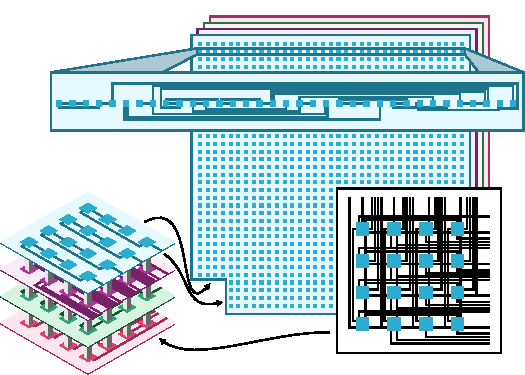
\includegraphics{figs/layout.pdf}
\end{frame}
